\documentclass[12pt, a4paper, oneside]{ctexart}
\usepackage{amsmath, amsthm, amssymb, appendix, bm, graphicx, hyperref, mathrsfs}
\usepackage{geometry}
\usepackage{algorithm}
\usepackage{algorithmicx}
\usepackage{algpseudocode}
\usepackage{amsmath}

\geometry{a4paper, left=2cm, right=2cm, top=2.5cm, bottom=2cm}

\title{\textbf{基于Francis QR算法的实Schur分解}}
\author{李维杰}
\date{\today}
\linespread{1.25}

\begin{document}

\maketitle

\pagenumbering{Roman}
\setcounter{page}{0}
\tableofcontents

\newpage
\setcounter{page}{1}
\pagenumbering{arabic}

\section{算法}

实现实Schur分解的代码框架如下:
\begin{algorithm}
    \caption{Real Schur Decomposition}
    \begin{algorithmic}[1]
        \Function{QR\_Iteration}{$M$}
            \State $r \gets n, l \gets 1$
            \State $[A, Q] \gets \text{Householder\_Hessenberg}(M)$ \Comment{Compute the Hessenberg form of $M$ and orthogonal matrix $Q$}

            \While{$r > l$}
                \State Eliminate small off-diagonal elements                
                \State $[isreal, eig_1, eig_2] \gets \text{eigen\_shift}(A(r-1:r, r-1:r))$ \Comment{Compute the eigenvalues of the current submatrix}
                \If{$isreal = 1$}
                    \State Choose the smaller eigenvalue $min\_eig$
                    \State $[A, Q] \gets \text{single\_shift\_iteration}(A, l, r, min\_eig, Q)$ \Comment{Perform a single shift iteration}
                \Else
                    \If{$r > l + 1$}
                        \State $[A, Q] \gets \text{double\_shift\_iteration}(A, l, r, eig_1 + eig_2, eig_1 \times eig_2, Q)$ \Comment{Perform a double shift iteration}
                    \Else
                        \State \textbf{Break} \Comment{Exit the loop if $r \leq l + 1$}
                    \EndIf
                \EndIf                
            \EndWhile
            \State \Return $A, Q$ \Comment{Return the computed matrix $A$ and orthogonal matrix $Q$}
        \EndFunction
    \end{algorithmic}
\end{algorithm}\\
具体来说,它由以下两步算法组成:

\subsection{基于Householder变换的矩阵上Hessenberg化}

对于任意给定的实矩阵$M \in \mathbb{R}^{n \times n}$, 我们采用Householder变换,第$k$步变换$HAH^T$将矩阵$A$的第$(k-1)$列的第$(k+1)$行及以下元素置零,从而将$A$阵变换为一个上Hessenberg阵.
这一部分算法的伪代码见附录A.

\subsection{上Hessenberg矩阵的实Schur分解}

对于上Hessenberg化的矩阵$A \in \mathbb{R}^{n \times n}$,将其分块为
\begin{align*}
    A = \left[
        \begin{array}{ccc}	
            T_{11} & T_{12} & T_{13} \\
                   & T_{22} & T_{23} \\
                   &        & T_{33}
        \end{array}
    \right],
\end{align*}
其中$T_{11},T_{33}$均是已完成收敛的拟上三角阵.这里$T_{11}$收敛为拟上三角阵是因为模数远大于其它特征值的特征值会提前收敛于左上角,$T_{33}$收敛为拟上三角阵是因为带位移的QR算法会不断把接近位移$\mu$的特征值收敛于右下角.
约定本节之后所提到的$A$均指代$T_{22}\in \mathbb{R}^{(r-l+1) \times (r-l+1)}$.计算该矩阵右下角$2 \times 2$子矩阵的特征值$\mu_1, \mu_2$. \par
(1) 当$\mu_1,\mu_2 \in \mathbb{R}$时,采用Wilkinson隐式位移.\par
取$\mu_1$与$\mu_2$中距离$A(r, r)$最近的一项作为位移量.在变换过程中,采用Givens变换逐一把下次对角线下方的bulge排出,从而完成一步迭代过程.特别地,由于隐式Q定理,第一步Givens变换矩阵$G_1$中的$c,s$应被确定为
\begin{align}
    \left\{
        \begin{array}{ll}
            c = \frac{A(1, 1) - \mu}{\sqrt{(A(1, 1) - \mu)^2 + A(2, 1)^2}} \\
            s = \frac{A(2, 1)}{\sqrt{(A(1, 1) - \mu)^2 + A(2, 1)^2}}
        \end{array}
    \right.
\end{align}
这一部分算法的伪代码见附录B.

(2) 当$\mu_1,\mu_2 \in \mathbb{C}$时,采用Francis隐式双位移.\par
使共轭复数$\lambda_1$与$\lambda_2$交替对矩阵$A$做位移.在变换过程中,采用Householder变换逐一把下次对角线下方的$2 \times 2$bulge排出,从而完成一步迭代过程(最后一步由于bulge只剩一个元素,故可以使用Givens变换).
特别地,由于隐式Q定理,第一步Householder变换矩阵应当将$e_1$镜射为向量$x$,其中$x$是向量$col_1(A^2-2\Re(\mu)A+|\mu|^2I)$的单位化结果.这一部分的伪代码见附录C.

\section{实现细节}
    \begin{enumerate}
        \item Francis QR算法可以被作用于任意实矩阵,算法过程中所有的计算均在实数域内进行.
        \item 算法中的所有Householder变换均由$(I-2\omega \omega^T)A = A - 2\omega(\omega^T A)$进行计算,从而绕过了求解Householder矩阵$H$的步骤.在这一优化下,所有Householder变换的效率均为$O(n^2)$.
        \item 为了进一步减小误差,在求位移时若发现右下角$2 \times 2$子矩阵的特征值为复数,则直接返回共轭特征值的和(即$\text{tr}(A(n-1:n, n-1:n))$)以及特征值的模长的平方(即$\det(A(n-1:n, n-1:n))$).
        \item 矩阵达到局部收敛的判断标准是:$$A(i+1,i) < \textbf{u} (|A(i+1, i+1)| + |(A(i, i))|),$$在满足这一条件时,置$A(i+1, i) = 0$, 并缩小参与迭代的子矩阵规模.
    \end{enumerate}

\section{数值表现}
    在对程序进行数值测试时,设定初始矩阵$M \in \mathbb{R}^{n \times n}$. 其中, $M$中的各元素在$(0,1)$中随机生成.
    在3.1至3.3小节中, 让$M$的规模$n$从$50$开始增长到$500$,对期间每一规模下的矩阵$M$进行Francis QR算法的数值测试;

\subsection{运行效率}
    Francis QR算法作用于各规模下的矩阵$M$时的运行效率表现如图1所示.可见运行效率-矩阵规模的对数图像近似线性,斜率对应于$O(n^3)$.

\subsection{数值稳定性}
    考察正交性损失${\left\lVert{Q^*Q - I}\right\rVert}_{\mathsf{F}}$和标准偏差$\frac{{\left\lVert{Q^* A Q - M}\right\rVert}_{\mathsf{F}}}{{\left\lVert{A}\right\rVert}_{\mathsf{F}}}$, 它们的数值表现如图2. 
    可见${\left\lVert{Q^*Q - I}\right\rVert}_{\mathsf{F}}$ 的数量级大约为$10^{-13}$,$\frac{{\left\lVert{Q^* A Q - M}\right\rVert}_{\mathsf{F}}}{{\left\lVert{A}\right\rVert}_{\mathsf{F}}}$的数量级大约为$10^{-7}$,二者均为极小量, 故可以认为Francis QR算法具有良好的数值稳定性.

    \begin{figure}[htbp]
        \centering
        \begin{minipage}{0.45\textwidth}
            \centering
            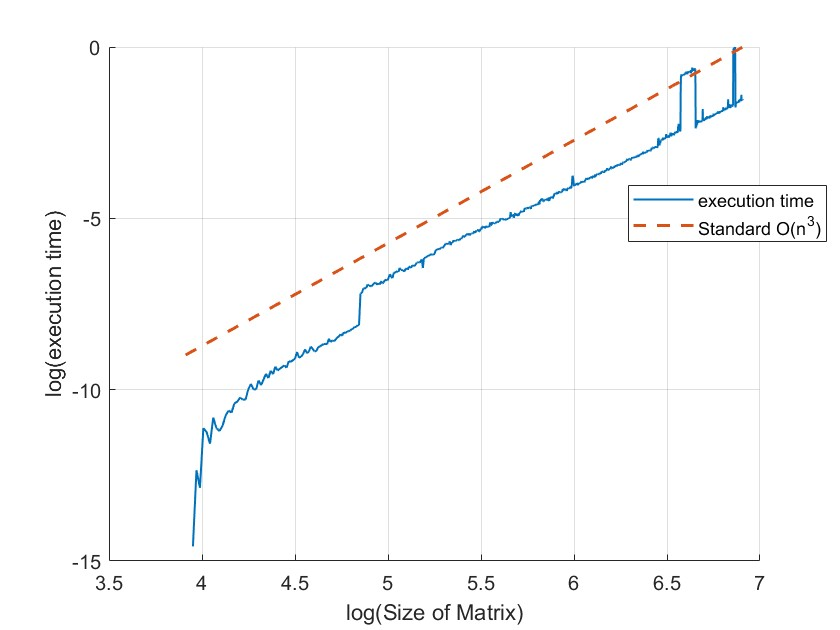
\includegraphics[scale=0.25]{execution time.jpg}
            \caption{运行时间}
        \end{minipage} 
        \hfill
        \begin{minipage}{0.45\textwidth}
            \centering
            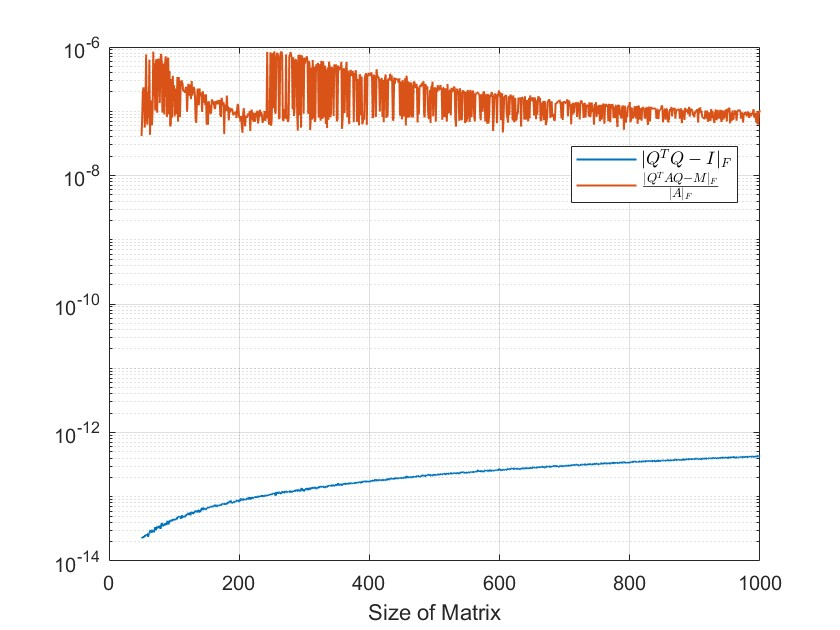
\includegraphics[scale=0.25]{error.jpg}
            \caption{数值稳定性}
        \end{minipage}
    \end{figure}

\subsection{迭代次数}
    由图3可见平均迭代$1.3$次即可得到一个特征值,即该算法具有相当快的收敛速度.

\subsection{收敛矩阵的结构}
    取规模为$2500$阶的初始矩阵$M$进行Francis QR算法, 最终得到的矩阵元素的热力图如图4, 可见这是一个拟上三角阵.\par
    \textbf{注:} 为了避免对角线上的元素过大导致上三角中的其它元素在热力图上的表现近似于$0$, 在绘制热力图时对角线上的元素均被做了缩小一定倍数的处理.

    \begin{figure}[htbp]
        \centering
        \begin{minipage}{0.45\textwidth}
            \centering
            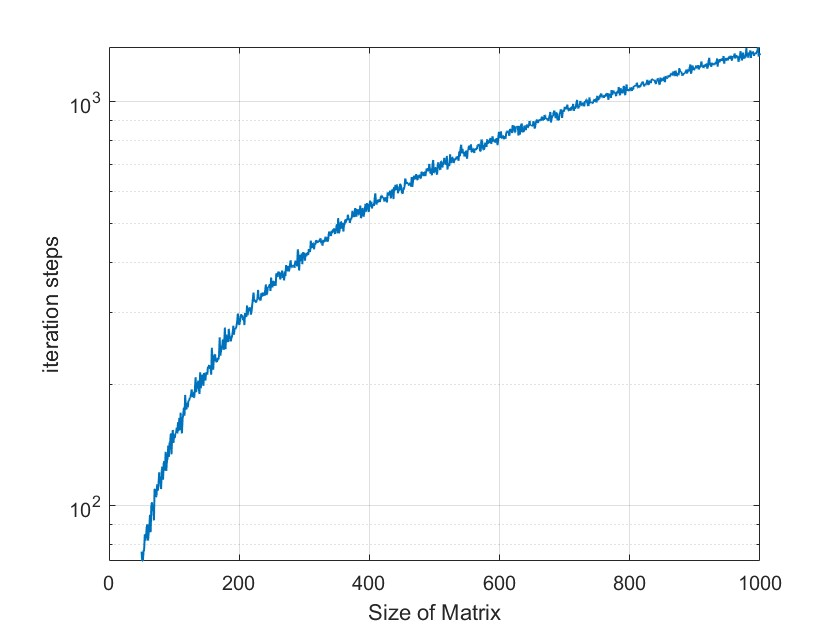
\includegraphics[scale=0.25]{iteration steps.jpg}
            \caption{迭代次数}
        \end{minipage} 
        \hfill
        \begin{minipage}{0.45\textwidth}
            \centering
            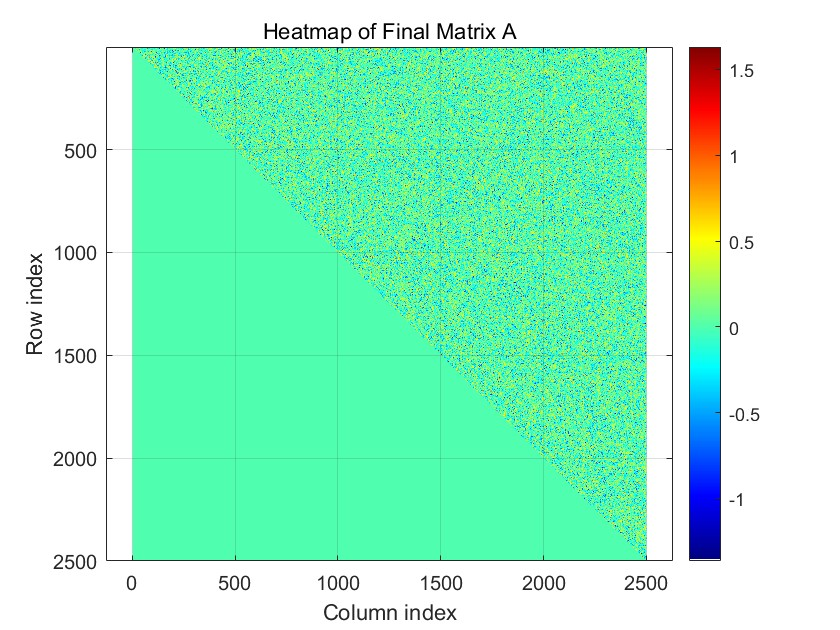
\includegraphics[scale=0.25]{structure.jpg}
            \caption{收敛矩阵结构}
        \end{minipage}
    \end{figure}
\newpage
\section{声明}
    在完成这份报告时,作者在以下方面使用了ChatGPT辅助作业:
    \begin{enumerate}
        \item 辅助将写好的代码转换为LaTeX格式的伪代码.
        \item 辅助撰写Matlab可视化数据的代码.
    \end{enumerate}
    除了上面提到的部分,其余内容均没有借用ChatGPT或其它可能的LLMs.

\begin{thebibliography}{99}
    \bibitem{a}徐树方,高立,张平文(2013). "数值线性代数(第二版)". 北京:北京大学出版社.
    \bibitem{b}https://www.cs.cornell.edu/~bindel/class/cs6210-f12/notes/lec28.pdf
    \bibitem{c}Trefethen, L. N., \& Bau, D. (1997). "Numerical linear algebra". Society for Industrial and Applied Mathematics.
    \bibitem{d}J.G.F. Francis, "The QR Transformation, I", The Computer Journal, 4(3), pages 265–271 (1961, received October 1959).
\end{thebibliography}

\newpage

\begin{appendices}
    \renewcommand{\thesection}{\Alph{section}}
    \section{基于Householder变换的矩阵上Hessenberg化}
    \begin{algorithm}
        \caption{Householder Transformation to Hessenberg Form}
        \begin{algorithmic}[1]
            \Require $M$: input matrix of size $n \times n$
            \Ensure Compute the Upper Hessenberg form of $M$ using Householder transformations
            \Function{Householder\_Hessenberg}{$A$}
                \State $n \gets$ number of rows (and columns) of $A$
                \For{$i = 1$ to $n - 2$}
                    \State $x \gets$ subvector of $A$ from row $i+1$ to $n$, column $i$
                    \State Compute the Householder matrix $H$ that sets $x$ to $e_1$
                    \State $A[i+1:n, i:n] \gets H \times A[i+1:n, i:n]$
                    \State $A[1:n, i+1:n] \gets A[1:n, i+1:n] \times H^T$
                \EndFor
                \State \Return $A$
            \EndFunction
        \end{algorithmic}
    \end{algorithm}
\end{appendices}
\newpage
\begin{appendices}
    \renewcommand{\thesection}{\Alph{section}}
    \section{Wilkinson隐式位移}
    \begin{algorithm}
        \caption{Single Shift Iteration with Givens Rotation}
        \begin{algorithmic}[1]
            \Require $A$: input matrix of size $n \times n$, $l$: the left side of the submatrix, $r$: the right side of the submatrix, $\mu$: shift parameter, $Q$: orthogonal matrix (initially identity matrix)
            \Ensure Compute the QR factorization of $A$ using Givens rotations with a single shift
            \Function{Single\_Shift\_Iteration}{$A, l, r, \mu, Q$}
                \State $[A, Q] \gets$ \textproc{Initial\_Givens}($A, l, r, \mu, Q$)
                \State $[A, Q] \gets$ \textproc{Givens\_Rotation}($A, l, r, Q$)
                \State \Return $A, Q$
            \EndFunction
        \end{algorithmic}
    \end{algorithm}
    \begin{algorithm}
        \caption{The first step of iteration}
        \begin{algorithmic}[1]
            \Function{Initial\_Givens}{$A, l, r, \mu, Q$}
                \State Compute the Givens matrix $G$ that satisfies the formula (1).
                \State $A(l:l+1, :) \gets G \times A(l:l+1, :)$
                \State $A(1:\min(l+2, r), l:l+1) \gets A(1:\min(l+2, r), l:l+1) \times G^T$
                \State $Q(l:l+1, :) \gets G \times Q(l:l+1, :)$
                \State \Return $A, Q$
            \EndFunction
        \end{algorithmic}
    \end{algorithm}
    \begin{algorithm}
        \caption{The Givens rotations during the iteration}
        \begin{algorithmic}[1]
            \Function{Givens\_Rotation}{$A, l, r, Q$}
                \State $n \gets$ size of $A$
                \For{$i = l$ to $r-2$}
                    \State Compute the Givens matrix $G$ that eliminates the bulge
                    \State $A(i+1:i+2, i:n) \gets G \times A(i+1:i+2, i:n)$
                    \State $A(1:\min(i+3, r), i+1:i+2) \gets A(1:\min(i+3, r), i+1:i+2) \times G^T$
                    \State $Q(i+1:i+2, :) \gets G \times Q(i+1:i+2, :)$
                \EndFor
                \State \Return $A, Q$
            \EndFunction
        \end{algorithmic}
    \end{algorithm}
\end{appendices}
\newpage
\begin{appendices}
    \renewcommand{\thesection}{\Alph{section}}
    \section{Francis隐式双位移}
    \begin{algorithm}
        \caption{Double Shift Iteration with Householder Reflection and Givens Rotation}
        \begin{algorithmic}[1]
            \Require $A$: input matrix of size $n \times n$, $l$: the left side of the submatrix, $r$: the right side of the submatrix, $m_{\text{real}}$: twice the real part of the shift, $m_{\text{norm}}$: norm of the shift, $Q$: orthogonal matrix
            \Ensure Compute the QR factorization of $A$ using Householder reflections and Givens rotations with double shift
            
            \Function{Double\_Shift\_Iteration}{$A, l, r, m_{\text{real}}, m_{\text{norm}}, Q$}
                \State $[A, Q] \gets$ \textproc{Initial\_Householder}($A, l, r, m_{\text{real}}, m_{\text{norm}}, Q$)
                \State $[A, Q] \gets$ \textproc{Householder\_Reflection}($A, l, r, Q$)
                \State $[A, Q] \gets$ \textproc{Givens\_Rotation}($A, l, r, Q$)
                \State \Return $A, Q$
            \EndFunction
        \end{algorithmic}
    \end{algorithm}

    \begin{algorithm}
        \caption{The first step of the iteration}
        \begin{algorithmic}[1]
            \Function{Initial\_Householder}{$A, l, r, m_{\text{real}}, m_{\text{norm}}, Q$}
                \State $n \gets$ the size of $A$
                \State $x \gets$ the first column vector of $A^2-2\Re(\mu)A+|\mu|^2I$
                \State Compute the Householder matrix P that sets $e_1$ to $x$
                \State $A(l:l+2, l:n) \gets P' \cdot A(l:l+2, l:n)$
                \State $A(1:\min(l+3, r), l:l+2) \gets A(1:\min(l+3, r), l:l+2) \cdot P$
                \State $Q(l:l+2, :) \gets P' \cdot Q(l:l+2, :)$
                \State \Return $A, Q$
            \EndFunction
        \end{algorithmic}
    \end{algorithm}

    \begin{algorithm}
        \caption{The Householder reflections during the iteration}
        \begin{algorithmic}[1]
            \Function{Householder\_Reflection}{$A, l, r, Q$}
                \State $n \gets$ the size of $A$
                \For{$i = l$ to $r - 3$}
                    \State Compute the Householder matrix $H$ that eliminates the bulge
                    \State $A(i+1:i+3, i:n) \gets H \cdot A(i+1:i+3, i:n)$
                    \State $A(1:\min(i+4, r), i+1:i+3) \gets A(1:\min(i+4, r), i+1:i+3) \cdot H'$
                    \State $Q(i+1:i+3, :) \gets H \cdot Q(i+1:i+3, :)$
                \EndFor
                \State \Return $A, Q$
            \EndFunction
        \end{algorithmic}
    \end{algorithm}

    \begin{algorithm}
        \caption{The Givens rotation at the end of the iteration}
        \begin{algorithmic}[1]
            \Function{Givens\_Rotation}{$A, l, r, Q$}
                \State $n \gets$ the size of $A$
                \State Compute the Givens rotation $G$ that eliminates the bulge
                \State $A(r-1:r, r-2:n) \gets G \cdot A(r-1:r, r-2:n)$
                \State $A(1:r, r-1:r) \gets A(1:r, r-1:r) \cdot G^T$
                \State $Q(r-1:r, :) \gets G \cdot Q(r-1:r, :)$
                \State \Return $A, Q$
            \EndFunction
        \end{algorithmic}
    \end{algorithm}
\end{appendices}
\newpage

\end{document}